\documentclass[10pt,conference,letterpaper]{IEEEtran}
\usepackage{verbatim}
\usepackage{moreverb}
\usepackage{url}
\usepackage{amsmath}
\usepackage{color}

\title{HAMAKE: A Dataflow Approach to Data Processing in Hadoop}

\begin{comment}

\author{\IEEEauthorblockN{Vadim Zaliva}
\IEEEauthorblockA{Codeminders\\
Email: lord@crocodile.org} \and \IEEEauthorblockN{Vladimir Orlov}
\IEEEauthorblockA{Codeminders\\
Email: vorl@codeminders.com}}
\end{comment}

\date{\today}
\usepackage{graphicx}
\usepackage{listings}
\usepackage[colorlinks=false,bookmarks=true,pdfauthor={Vadim Zaliva lord@crocodile.org, Vladimir Orlov vorl@codeminders.com},
            pdftitle={HAMAKE: A Dataflow Approach to Data Processing in Hadoop},
            pdftex]{hyperref}

% graphviz.tex
% originally written by Derek Rayside, November 2003
% following an idea that Daniel Jackson implemented in his Tagger program
%
% parameters to \digraph:
% 1 - parameters for \includegraphics (optional; default value is "scale=1")
% 2 - name of the digraph
% 3 - body of the digraph

\newcommand{\digraph}[3][scale=1]{
    \newwrite\dotfile
    \immediate\openout\dotfile=#2.dot
    \immediate\write\dotfile{digraph #2 {\string#3}}
    \immediate\closeout\dotfile
    \IfFileExists{#2.ps}
        % the postscript exists: include it
        { \includegraphics[#1]{#2} }
        % the postscript doesn't exist: tell the user how to create it
        { \fbox{ \begin{tabular}{l}
            The file \texttt{#2.ps} hasn't been created from
            \texttt{#2.dot} yet. \\
            Run `\texttt{dot -Tps -o #2.ps #2.dot}' to create it. \\
            Here is a \textsf{bash} loop to process all \textsf{dot} files
            in the current directory: \\
            \texttt{
            for f in *.dot do ; 
            dot -Tps -o \$\{f\%dot\}ps \$f ; 
            done
            }
            \end{tabular}}
        }
}


\begin{document}
\lstset{language=XML,basicstyle=\tiny,markfirstintag=true,numbers=left,numbersep=1pt}

\maketitle

\begin{abstract}
  Most non-trivial data processing scenarios using Hadoop typically
  involve launching more than one MapReduce job. Usually, such
  processing is data-driven with the data funneled through a sequence
  of jobs.  The processing model could be expressed in terms of
  dataflow programming, represented as a directed graph with datasets
  as vertices. Using \textit{fuzzy timestamps} as a way to detect
  which dataset needs to be updated, we can calculate a sequence in
  which Hadoop jobs should be launched to bring all datasets up to
  date. Incremental data processing and parallel job execution fit
  well into this approach.

  These ideas inspired the creation of the \textbf{hamake} utility.    We attempted to emphasize data allowing the developer to formulate
  the problem as a data flow, in contrast to the workflow
  approach commonly used. \textbf{Hamake} language uses just two data
  flow operators: \emph{fold} and \emph{foreach}, providing a clear
  processing model similar to MapReduce, but on a dataset level.
\end{abstract}

\section{Motivation and Background}

Hadoop\cite{bialecki2005hadoop} is a popular  open-source implementation of MapReduce, a data processing model introduced by Google\cite{dean2008map}.

Hadoop is typically used to process large amounts of data through a series of relatively simple operations. Usually Hadoop jobs are I/O-bound
\cite{hadoopattwitter,hs2010hadoopbench}, and execution of even
trivial operations on a large dataset could take significant system
resources. This makes incremental processing especially important. Our initial
inspiration was the Unix \emph{make} utility. While applying some of the ideas implemented by \emph{make} to Hadoop, we took the opportunity to generalize the processing model in terms of dataflow programming.

\textbf{Hamake} was developed in late 2008 to address the problem of
incremental processing of large data sets in a collaborative filtering project.

We've striven to create an easy to use utility that developers can
start using right away without complex installation or extensive
learning curve. 

\begin{comment}
\textbf{Hamake} is open source and is distributed under Apache
License v2.0. The project is hosted at Google Code at the following
URL: \url{http://code.google.com/p/hamake/}.
\end{comment}


\section{Processing Model}

\textbf{Hamake} operates on \textit{files} residing on a local or
distributed file system accessible from the Hadoop job. Each file has a timestamp reflecting the date and time of its
last modification. A file system directory or folder is also a file
with its own timestamp. A \textit{Data Transformation Rule (DTR)}
defines an operation which takes files as input and produces other
files as output.

If file \textit{A} is listed as input of a DTR, and file \textit{B}
is listed as output of the same DTR, it is said that \textit{``B depends
  on A.''} \textbf{Hamake} uses file time stamps for dependency
up-to-date checks. DTR output is said to be \textit{up to date} if the minimum time stamp on all outputs is greater than or equal to the maximum timestamp on all inputs. For the sake of convenience, a user could arrange groups of files and folders into a \emph{fileset} which could later be referenced as the DTR's input or output.

\textbf{Hamake} uses \textit{fuzzy timestamps}\footnote{The current stable
  version of \textbf{hamake} uses exact (non-fuzzy) timestamps.}
which can be compared, allowing for a slight margin of error. The
``fuzziness'' is controlled by a tolerance of $\sigma$. Timestamp $a$ is considered to be older than timestamp $b$ if $(b-a)>\sigma$. Setting $\sigma=0$ gives us a non-fuzzy, strict timestamp comparison.

\textbf{Hamake} attempts to ensure that all outputs from a DTR are up to
date\footnote{Because \textbf{hamake} has no way to update them, it does not attempt to ensure that files are up to date, unless they are listed as one of a DTR's outputs.} To do so, it builds a \textit{dependency graph} with DTRs as edges and individual files or filesets as vertices. Below, we show that this graph is guaranteed to be a \textit{Directed Acyclic Graph} (DAG).

After building a \textit{dependency graph}, a graph reduction algorithm (shown in Figure~\ref{fig:grred}) is executed. Step 1 uses Kahn's algorithm\cite{kahn1962topological} of topological ordering. In step 6, when the completed DTR is removed from the dependency graph, all edges pointing to it from other DTRs are also removed.

\begin{figure}[htp]
\centering
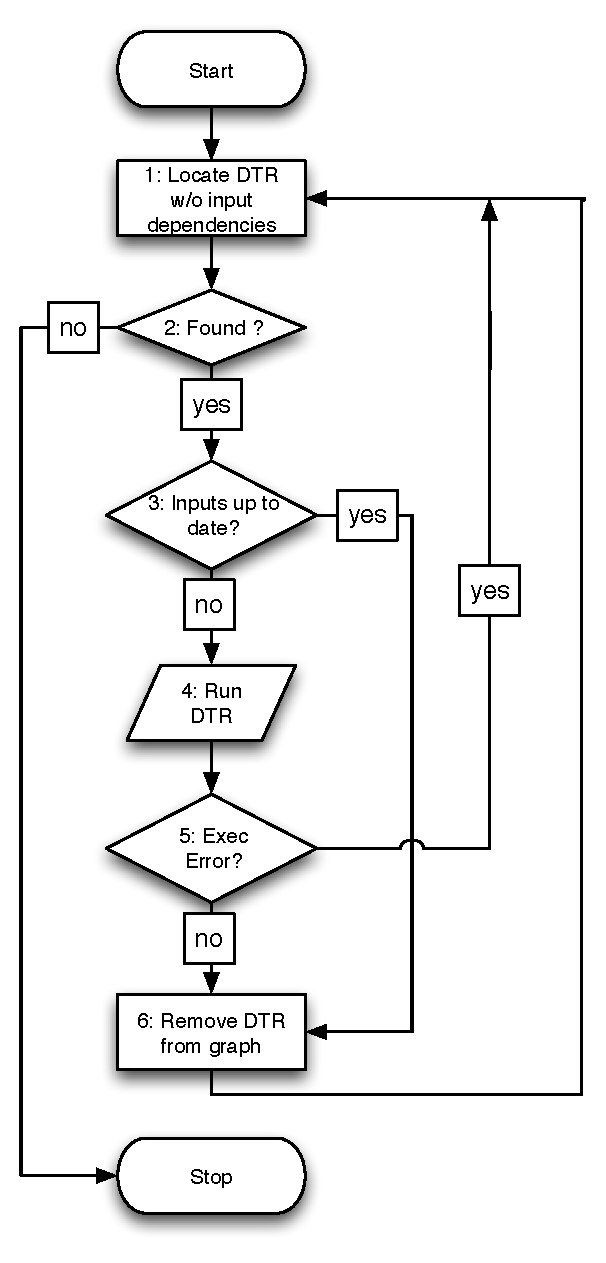
\includegraphics[width=4cm]{GraphReduction.eps}
\caption{\textbf{hamake} dependency graph reduction algorithm}
\label{fig:grred}
\end{figure}

The algorithm allows for parallelism. If more than one DTR without
input dependencies is found during step 1, the subsequent steps 2-6 can be executed in parallel for each discovered DTR.

It should be noted that if DTR exectuion has failed, \textbf{hamake} can and will continue to process other DTRs which do not depend directly or indirectly on the results of this DTR. This permits the user to fix problems later and re-run \textbf{hamake}, without the need to re-process all data.

Cyclic dependencies must be avoided, because a dataflow containing
such dependencies is not guaranteed to terminate. Implicit checks are performed during the reading of DAG definitions and the building of the dependency graph. If a cycle is detected, it is reported as an error. Thus the dependency graph used by \textbf{hamake} is assured to be a \textit{directed acyclic graph}.

However, \textbf{hamake} supports a limited scenario of iterative
processing with a feature called \textit{generations}. Each input or
output file can be marked with a \emph{generation}
attribute. Any two files referencing the same path in the file system while having different generations are represented as two distinct vertices in the dependency graph. This permits resolution of cyclic dependencies within the context of a single \textbf{hamake} execution.

One useful consequence of \textbf{hamake} dataflow being a DAG is
that for each vertex we can calculate the list of vertices it depends on directly and indirectly using simple \textit{transitive closure}. This allows us to easily estimate the part of a dataflow graph being affected by updating one or more files, which could be especially useful for datasets where the cost of re-calculation is potentially high due to data size or computational complexity. 

\textbf{Hamake} is driven by dataflow description, expressed in a simple XML-based language. The full syntax is described in
\cite{hamakesyntax}. The two main elements, \emph{fold} and \emph{foreach}, correspond to two types of DTRs. Each element has input, output, and processing instructions. The execution of processing instructions brings the DTR output up to date. 

\emph{Fold} implies a many-to-one dependency between input and output. In other words, the output depends on the entirety of the input, and if any of the inputs have been changed, the outputs need to be updated. \emph{Foreach} implies a one-to-one dependency where for each file in an input set there is a corresponding file in an output set, each updated independently.

\textbf{Hamake} dataflow language has declarative semantics making it easy to implement various dataflow analysis and optimization algorithms in the future. Examples of such algorithms include: merging dataflows, further execution parallelization, and analysis and estimation of dataflow complexity.

\section{Parallel Execution}

While determining the sequence and launching of Hadoop jobs required to bring all datasets up-to-date, \textbf{hamake} attempts to perform all required computations in the shortest possible time. To achieve this, \textbf{hamake} aims for maximal cluster utilization, running as many Hadoop jobs in parallel as cluster capacity permits.

There are three main factors that drive job scheduling logic: file
timestamps, dependencies, and cluster computational capacity. On the
highest level, DTR dependencies determine the sequence of jobs to be 
launched.

In the case of \emph{fold} DTR, a single Hadoop job, PIG script or
shell command, may be launched, and hence there is no opportunity for parallel execution. In the example shown in
Figure~\ref{fig:fold2}, since fileset \textit{B} depends on all files in fileset \textit{A}, a single job associated with \emph{fold} DTR will be executed.

\begin{figure}[htp]
\centering
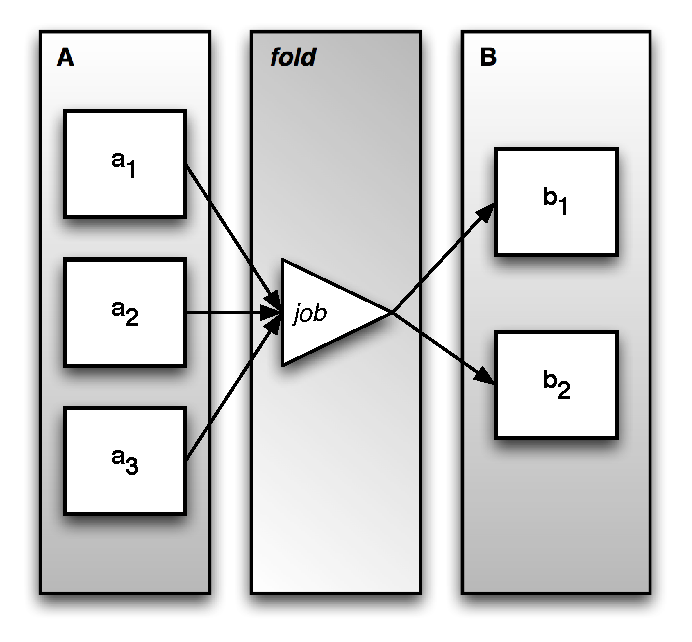
\includegraphics[width=0.3\textwidth]{twofoldp.eps}
\caption{Decomposition of \emph{fold} DTR}
\label{fig:fold2}
\end{figure}

A \emph{foreach} DTR works by mapping individual files in fileset
\textit{A} to files in fileset \textit{B}. Assuming that fileset
\textit{A} consists of 3 files: \textit{$a_1$}, \textit{$a_2$},
\textit{$a_3$}, the dependency graph could be represented as shown
in Figure~\ref{fig:foreach2}. In this case, we have an opportunity to execute the three jobs in parallel.

\begin{figure}[htp]
\centering
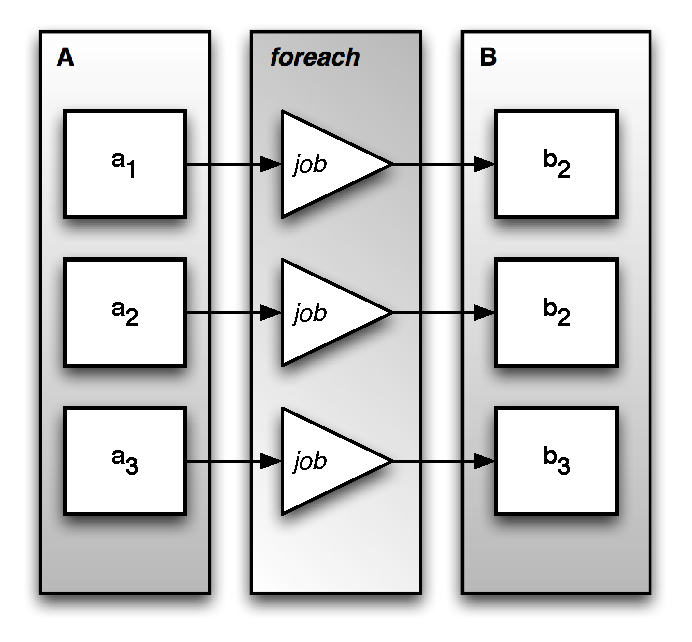
\includegraphics[width=0.3\textwidth]{twoforeachp.eps}
\caption{Decomposition of \emph{foreach} DTR}
\label{fig:foreach2}
\end{figure}

The Hadoop cluster capacity is defined in terms of the number of
\textit{map slots} and \textit{reduce slots}. When a DTR launches a
Hadoop job, either directly as defined by \emph{mapreduce} processing instruction or via PIG script, a single job will spawn one or more \emph{mapper} or \emph{reducer} tasks, each taking one respective slot. The number of mappers and reducers launched depends on many factors, such as the size of the HDFS block, Hadoop cluster settings, and individual job settings. In general, \textbf{hamake} has neither visibility of nor control over most of these factors, so it does not currently  deal with individual tasks. Thus \textbf{hamake} parallel
execution logic is controlled by a command line option specifying how many jobs it may run in parallel.

\section{Example}

In a large, online library, the \textbf{hamake} utility can be used to automate searches for duplicates within a corpus of millions of digital text documents. Documents with slight differences due to OCR errors, typos, differences in formatting, or added material such as a foreword or publisher’s note can be found and reported.
 
To illustrate \textbf{hamake} usage, consider the simple approach of using the \textit{Canopy clustering algorithm}\cite{efficientClustering} and a \textit{vector space model}\cite{manning2008introduction} based on word frequencies. The implementation could be split into a series of steps, each implemented as \textit{MapReduce job}:

\begin{description}[\IEEEsetlabelwidth{\emph{FilterStopwords}}]
\item[\emph{ExtractText}] Extract a plain text from native document format
  (e.g. PDF).
\item[\emph{Tokenize}] Split plain text into tokens which roughly
  correspond to words. Deal with hyphens, compound words,
  accents, and diacritics, as well as case-folding, stemming, or lemmatization, resulting in a list of normalized \text{tokens}.
\item[\emph{FilterStopwords}] Filter out \textit{stopwords}, 
  like \textit{a}, \textit{the}, and \textit{are}.
\item[\emph{CalculateTF}]  Calculate a feature vector of term frequencies for each document.
\item[\emph{FindSimilar}] Run \textit{Canopy clustering algorithm}
  to group similar documents into clusters using
  \textit{cosine distance} as a fast approximate distance metric. 
\item[\emph{OutputResult}] Output document names, which are found in
  clusters with more than one element.
\end{description}

Each of the six MapReduce jobs produces an output file which
depends on its input. For each document, these jobs must be invoked
sequentially, as the output of one task is used as input of the next. Additionally, there is a configuration file containing a list of
stop words, and some task outputs depend on this file content. These
dependencies could be represented by a DAG, as shown in Figure~\ref{fig:SimilarityAlgDAG}, with vertices representing documents and jobs assigned to edges. The XML file describing this dataflow in \textbf{hamake} language is shown as
Listing~\ref{hamakeFile}.

\lstinputlisting[caption={\textit{hamakefile}, describing process for detecting duplicate documents}, label=hamakeFile]{sample.xml}

The first DTR (lines 10-25) converts a document from a native format such
as PDF to plain text. The input of the DTR is a reference to the
\emph{/doc} folder, and the output is the \emph{/txt} folder. The
\emph{foreach} DTR establishes one-to-one dependencies between files
with identical names in these two folders. The Hadoop job which
performs the actual text extraction is defined using the \emph{mapreduce}
element. It will be invoked by \textbf{hamake} for each unsatisfied
dependency. The job takes two parameters, defined with
\emph{parameter} elements - a path to an original document as the input and a path to a file where the plain text version will be written. The remaining five DTRs are defined in a similar manner.

\textbf{Hamake}, when launched with this XML dataflow definition, will execute a graph reduction algorithm, as shown in Figure~\ref{fig:grred}, and will find the first DTR to process. In our example, this is
\emph{ExtractPlainText}. First, \textbf{Hamake} will launch the  corresponding Hadoop job and immediately following, execute DTRs which depend on the output of this DTR, and so on until all output files are up to date. As a result of this data flow, a file named
\emph{results.txt} with a list of similar documents will be generated.

This data flow could be used for incremental processing. 

When new documents are added, \textbf{hamake} will refrain from running the following DTRs: \emph{ExtractText}, \emph{Tokenize}, \emph{FilterStopWords}, and \emph{CalculateTF} for previously processed documents. However, it will run those DTRs for newly added documents and then, re-run \emph{FindSimilar} and \emph{OutputResults}. 

If the list of stop
words has been changed, \textbf{hamake} will re-run only
\emph{FilterStopWords}, \emph{CalculateTF}, \emph{FindSimilar}, and
\emph{OutputResults}.

\begin{figure}[htp]
\centering
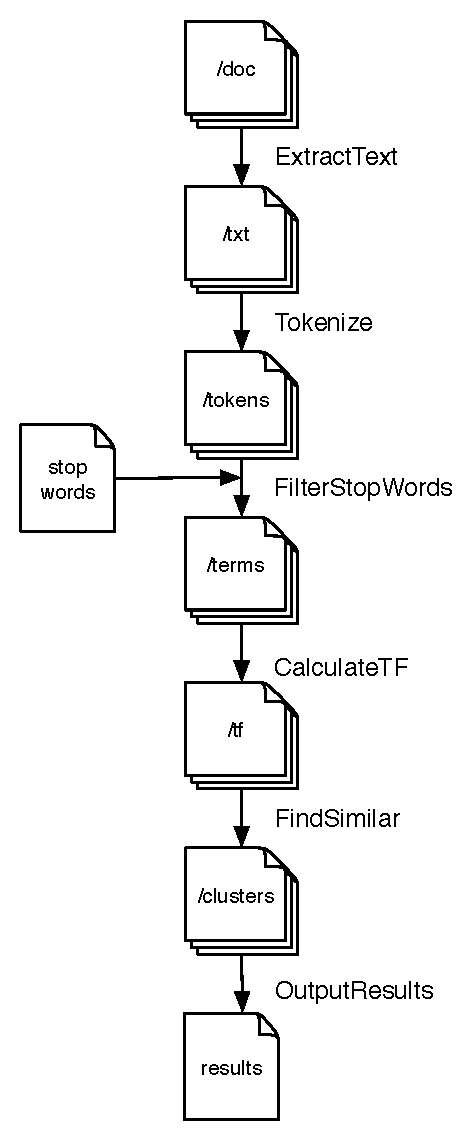
\includegraphics[width=0.25\textwidth]{SimilarityAlgDAG.eps}
\caption{Directed acyclic graph of a data flow for duplicate document detection}
\label{fig:SimilarityAlgDAG}
\end{figure}

\section{Related Work}

Several workflow engines exist for Hadoop, such as
\href{http://github.com/tucu00/oozie1}{Oozie},
\href{http://sna-projects.com/azkaban/}{Azkaban}, and
\href{http://www.cascading.org/}{Cascading}.  Although all of these
products could be used to solve similar problems, they differ
significantly in design, philosophy, target user profile, and usage
scenarios limiting the usefulness of a simple, feature-wise
comparison.

The most significant difference between these engines and \textbf{hamake}
lies in the \textit{workflow} vs. \textit{dataflow} approach. All of them
use the former, explicitly specifying dependencies between
jobs. \textbf{Hamake}, in contrast, uses dependencies between datasets to derive workflow. Both approaches have their advantages, but for some problems, the dataflow representation as used by
\textbf{hamake} is more natural.

\section{Future Directions}

One possible \textbf{hamake} improvement may be better integration with Hadoop schedulers. For example, if \textit{Capacity Scheduler} or \textit{Fair Scheduler} is used, it would be useful for \textbf{hamake} to take information about scheduler \textit{pools} or \textit{queues} capacity into account in its job scheduling algorithm.

More granular control over parallelism could be achieved if the
\textbf{hamake} internal dependency graph for \emph{foreach} DTR
contained individual files rather than just filesets. For example, consider a
dataflow consisting of three filesets \textit{A}, \textit{B},
\textit{C}, and two \emph{foreach} DTR's: \textit{$D_1$}, mapping
\textit{A} to \textit{B}, and \textit{$D_2$}, mapping \textit{B} to
\textit{C}. File-level dependencies would allow some jobs to run from
\textit{$D_2$} without waiting for all jobs in \textit{$D_1$} to
complete.

Another potential area of future extension is the \textbf{hamake} dependency
mechanism. The current implementation uses a fairly simple timestamp
comparison to check whether dependency is satisfied. This could be
generalized, allowing the user to specify custom dependency check
predicates, implemented either as plugins, scripts 
(in some embedded
scripting languages), or external programs. This would allow for
decisions based not only on file meta data, such as the timestamp, but also on its contents.

Several \textbf{hamake} users have requested support for iterative computations with a termination condition. Possible use-cases include fixed-point computations and clustering or iterative regression algorithms. Presently, to embed this kind of algorithm into the \textbf{hamake} dataflow, it requires the use of the \textit{generations} feature combined with external automation, which invokes \textbf{hamake} repeatedly until a certain exit condition is satisfied. \textbf{Hamake} users could
certainly benefit from native support for this kind of dataflow.

\bibliography{hamake}
\bibliographystyle{unsrt}

\end{document}

